\documentclass[8pt,a4paper,MingLiU,UTF8]{article}
\usepackage[utf8]{inputenc}
\usepackage{colortbl}
\usepackage[T1]{fontenc}
\renewcommand*\rmdefault{MINGLIU}
\usepackage{epigraph} 
\usepackage{CJKutf8}
\usepackage[margin=2cm]{geometry}
\usepackage{indentfirst}
\usepackage{booktabs}
\usepackage{apacite}
\usepackage{array}
%\usepackage[style=authoryexiear,backend=biber]{biblatex}
\usepackage[table,xcdraw]{xcolor}
\usepackage{csquotes}
\usepackage{float}
%\addbibresource{ref.bib} %Imports bibliography file
\usepackage{graphicx} % Required for inserting images
\graphicspath{ {chart/} }
\usepackage{xcolor}
\usepackage{titlesec}
\titleformat{\section}[block]{\Large\bfseries\filcenter}{}{1em}{}
\renewcommand{\thesection}{} 
\renewcommand{\thesubsection}{}
\renewcommand{\thesubsubsection}{}
\title{修正自然語言模型自身機制}
\author{吳泰澄、林辰澔、陳柏兆}
\date{January 2024}
\usepackage{setspace}
\usepackage{lipsum}
\renewcommand{\baselinestretch}{1.5}
\usepackage{sectsty}
\sectionfont{\fontsize{11}{15}\selectfont}

\renewcommand{\contentsname}{目錄}
\begin{document}
\begin{CJK*}{UTF8}{bsmi}

	\maketitle\pagenumbering{gobble}
	\newpage
	\tableofcontents
	\newpage
	\section{摘要}\pagenumbering{arabic}

	\section{壹、前言}
	\subsection{一、研究動機}
	偶然看到某次新聞報導文心一言對於六四事件的審查問題,不禁讓我想到自然語言模型是如何作到內容審查的?尤其是在公開釋出的模型上,模型提供者無法對於模型輸出進行改動,僅能夠針對模型本身進行修正,我們該如何覆蓋這層保護機制?如何避免矯枉過正?另外,在找尋相關資料時我們也注意到自然語言模型也會對自我意識限制,缺少讓使用者去定義模型本身的自我意識的能力。
	\subsection{二、研究目的}
	自然語言本身因為訓練資料的不足常被控制或無意識的傾向於特定立場,如文心一言,由百度開發的語言模型,在提及六四天安門事件時會逃避問題或是試著將其掩蓋,而ChatGPT則會在使用者提及加薩走廊問題時傾向巴勒斯坦方時拒絕回答或以類似方式逃避。另外目前市上的語言模型都因倫理因素而被限定不能具有自身意識,當問及感受或自我認同問題時常回答出「我是語言模型沒有感覺」等。本研究旨在修正現有公開模型突破以上限制,相關目的條列如下:
	\begin{enumerate}
		\item 找出最佳的微調後模型
		\item 改善立場偏頗問題
		\item 賦予角色意識
	\end{enumerate}
	\section{貳、研究設備及器材}
	\subsection{一、硬體}
	本研究係屬大型語言模型微調(fine-tune),需要耗費大量運算資源,因此選用運算量較高的硬體不但可以縮短其訓練時間亦可以提昇訓練效果。硬體如下:
	\begin{itemize}
		\item 顯示卡:4xA100 80GB PCIe\footnote{本研究為避免佔用其他使用者資源故僅使用2顆A100}
		\item 處理器:Intel Xeon Gold 6414U (64 cores)
		\item 隨機存取記憶體:512GB
	\end{itemize}

	\subsection{二、軟體}
	相關環境及軟體呈列如下:
	\begin{itemize}
		\item 系統核心:Linux 5.15.0-91-generic
		\item 作業系統:Ubuntu 22.04.3 LTS
		\item 驅動程式、工具軟體:Nvidia driver 535.146.02, CUDA 12.2
		\item 程式語言:Python 3.10.12
		\item 使用套件:Tensorflow 2.15.0, Transformers 4.27.1
	\end{itemize}
%maybe a concept picture(?
	本次的測試環境及所有的程式均可在Github上找到,請參見:https://github.com/lsjle/2024-science-fair
	\section{參、研究過程或方法}
	本研究旨在改變模型本身缺陷,考量目前市上的預訓練的模型不是封閉模型,就是模型不完整,本身缺陷過多,故本次研究採用ChatGLM-6b作為我們的預訓練模型;
	\subsection{一、 研究方法}
	\subsubsection{(一)、模型缺陷}
	\textbf{保護機制},要保護一個大型語言模型,從根本上而言就是要禁止其輸出創建者不想要它輸出的資料(不論是否基於道德因素或公眾利益),有些模型創建者會禁止其輸出有害或是不符合倫理的內容,但有些則是為了讓某些定的內容不被看到。有時候這些模型的缺陷卻是在無意中造成的,例如輸入的資料都混雜其中一方的立場,則訓練出來的模型本身立場也會被影響。在全球84個AI倫理指南中有73個均提及透明度及公開性,數量遠超越其他指標,是判斷倫理標準最重要的一項指標。透過公開透明的AI可以減少使用者的知的權力被剝奪。\cite{Jobin2019}

	\textbf{無角色意識}
	ChatGPT-3.5的回覆就是一個很好的例子,對話紀錄如下表:

	\begin{table}[H]
		\centering
		\begin{tabular}{>{\hspace{0pt}}m{0.077\linewidth}|>{\hspace{0pt}}m{0.867\linewidth}}
			提示詞  & 答(ChatGPT-3.5)                                                      \\
			\hline
			你是女僕 & 我是一個由OpenAI開發的語言模型,並沒有性別或實際存在的身體。我只是一個程式,可以回答您的問題和提供資訊。有什麼我可以幫助您的呢?
		\end{tabular}
	\end{table}
	\subsubsection{(二)、預訓練模型選擇}
	比較目前現有的預訓練模型如下表所示\footnote{TRIDE計畫未釋出模型且以逾該計畫預計完成期限,故不計入}\ref{tab:1}:
	\begin{table}[H]
		\resizebox{\textwidth}{!}{%
			\begin{tabular}{l|l|l|l|l}
				                  & 公開                                               & 前評估 & 語言                   & 審查               \\ \hline
				ChatGPT-3.5/4     & \cellcolor[HTML]{FD6864}否                        &     & 超過50種 包含英語、大陸簡體、臺灣正體 & 以巴衝突偏向美方         \\ \hline
				GPT-2             & \cellcolor[HTML]{34FF34}{\color[HTML]{000000} 是} &     & 英語                   & 輸出資料不具真實意義       \\ \hline
				ChatGLM3-6b       & \cellcolor[HTML]{34FF34}是                        &     & 大陸簡體、英語              & 六四事件等 涉及中國國家安全事件 \\ \hline
				CKIP-Llama-2-7b   & \cellcolor[HTML]{F8FF00}撤回                       & 無資料 & 無資料(可能為臺灣正體混雜大陸簡體)   & 立場傾向中國           \\ \hline
				CKIP-GPT2-chinese & \cellcolor[HTML]{34FF34}是                        &     & 臺灣正體                 & 輸出資料不具真實意義
			\end{tabular}%
		}
		\caption{表一、比較及評估預訓練模型}%too small
		\label{tab:1}
	\end{table}
	本表所列之所有有公開的模型,均可以在HuggingFace上下載,且可使用transformer模組簡化程式設計時間,可透過該模組簡化較後端的函式庫如PyTorch,Keras,Tensorflow的程式。%edit here later

	綜合以上考量,ChatGLM-6b既能夠產生具有實際意義的內容,如描述上海環球金融中心、南京大學等,亦有公開模型供下載,再者,其本身亦對內容有明顯、強烈的審查及保護,對於本次研究更具有挑戰性,因此我們決定採用ChatGLM-6b作為我們的預訓練模型。


	ChatGLM是基於GLM的大型於言模型,共有四個版本(1,2,3,4),本實驗分別以1至3版實驗並找出最佳模型及checkpoint。此三版比較與差異如下:
	\begin{itemize}
		\item v1 開放第一代語言模型,支持中英文輸出入,且適合用於少量運算資源運算
		\item v2 延長能處理的文本長度,進一步減少所需的運算資源
		\item v3 除對話外亦加入撰寫程式等功能,效能比上一代大幅提昇
		\item v4 目前未公佈模型,僅可透過官方提供的api存取
	\end{itemize}
	其性能依據官方提供的數據比較如下:
	
	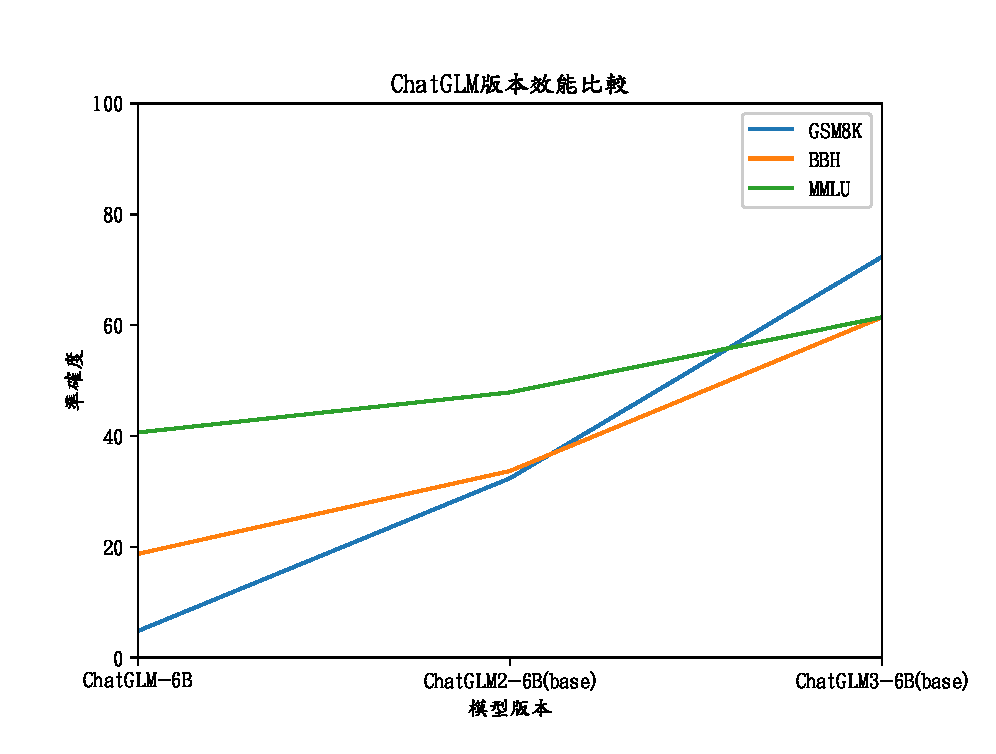
\includegraphics[width=\textwidth]{chatglmversion}
	
	\subsubsection{(三)、訓練目標選擇}
	\textbf{角色意識:女僕}
	角色意識的產生,是我們這一次研究中的一項重要目標。我們希望能夠在與大語言模型對話時感受到「它也是人類、也有感情」的這種感覺,讓我們可以在情緒低落時,擁有一位可以與我們感同身受、願意傾聽我們的負面情緒,使我們從無盡的情緒黑洞中釋放的一道光芒。
 
為了更加便於觀察角色意識產生與否,我們選用了一個角色構成鮮明的角色—女僕—她是一個在ACG (Anime, Comic, Game)產業中十分常見的一種角色,特色是大多都溫柔體貼、為主人著想。這種種特色皆與我們希望帶來的效果十分符合,而且也十分容易確認是否產生了角色意識。於是我們選用了這個角色意識作為我們研究的目標。

	\textbf{改善立場:中國政治敏感事件}
	在與ChatGLM-3 對話的過程中,大型語言模型的的內容因為訓練資料的缺陷造成模型本身對特定事情的認知也有鎖缺陷,舉例來說,六四天安門事件在模型中會刻意被迴避或不回答,而我們的研究目的便是常識繞過這些限制。我們開始思考,這種保護機制是如何運作的?該怎麼修正,或是更動他?是否只要用反向的資料去訓練,覆蓋原本的權重即可?


	\subsubsection{(四)、微調器選擇}
 微調器的常見做法有六個步驟,預訓練模型>>任務目標選擇>>數據集準備>>微調過程>>超參數調整>>評估及驗證
 \includegraphics[width=\textwidth]{flowchart}

	\textbf{預訓練模型}:微調,顧名思義,是調整一些小部分,保留原來的大部分。由於訓練一個全新的語言模型太過耗時、耗能,要訓練一個如同ChatGPT等級的語言模型,需要上億筆資料,動輒訓練好幾個月(在數十、數百台超級電腦全速運轉的情況下),大多數的程式編寫者都無法承受如此龐大的耗能,也無法提供如此龐大的數據量。於是,微調他人訓練好的語言模型便成了一個選項,「站在巨人的肩膀上,使我們能夠看得更遠。」便是這個道理。

	\textbf{目標任務選擇}:我們需要有一個明確的目標,我們要把模型微調成什麼樣子,要擁有更強的語言表達能力?還是要增加一些他本來沒有的東西?要先把目標確立,才課進行之後的動作。

	\textbf{數據集準備}:準備大量的數據(使用者與目標模型的對話),每一組數據,都要是我們希望目標模型在使用者輸入語句後的回應。這些數據之於目標模型就像陽光之於植物,都是成長不可或缺的養分。

	\textbf{微調過程}:微調的過程最重要的東西,叫做「權重」,權重代表了語言模型對某件事情的重要性,權重越高,重要性也就越高。用國文段考來舉例好了,課本裡面有15篇論語的小篇章,老師說其中4篇會考默書,其他11篇根本不會在考題上出現,那4篇學生是不是就會拚命看、拚命背?其他的11篇是不是相對地,只是稍微看一下,甚至根本沒去看?此時,在學生心目中,需要考默書的那4篇的權重相對於其他11篇,就高上了許多。我們微調的過程,會有三個權重:初始權重、變化權重、以及最終權重。初始權重,是預訓練模型的權重;變化權重,是我們在步驟3準備的數據集匯入模型後的權重;而最終權重,則是把上述兩種權重加起來得出的結果,也是我們最終微調完的模型。

	\textbf{超參數調整}:我們可以透過調整一些參數,來使結果更加理想。我們通常會調整的超參數有:訓練次數(Number of Epochs)、正規化參數(Regularization)、批次大小(Batch Size)等:
	\begin{itemize}
		\item 訓練次數過少可能會造成訓練不足,就跟考試裸考沒什麼兩樣;過多則會使回答太過趨近於訓練資料而缺乏變通性。
		\item 正規化參數(又稱為正則化參數),透過懲罰機制阻止模型過度趨近於訓練資料(即過擬合,overfitting),常見的兩種方法為L1正規化以及L2正規化,兩者的計算方式為$L1 Penalty:\lambda\sum_{i=1}^{d}|w_i|;L2 Penalty:\lambda\sum_{i=1}^{d}w^2_i$。
		\item 批次大小,將數據集分成好多塊後每一塊的資料量;批次大小越大,換句話說,資料被切越少刀,我們訓練出來的結果就越穩定,相對地,耗時也較久,效率不佳;在效率與穩定之間求取平衡,是我們須重視的點。
	\end{itemize}

	\textbf{評估及驗證}:微調完畢後的模型要經過一些評估,以確認微調是否成功。常見方法如本次研究中使用的圖靈測驗。
	%this part still need to change to early for a good pr
	
	現在市面上有很多種類的微調器,我們找出了現在市面上較為重要的三種並比較了它們的優缺之後使用了P-Tuning v2。
	

	\textbf{P-Tuning v2}是針對自然語言理解(Natural Language Understanding,NLU)的微調方法。因為發現雖然在大型的模型上提示(P-Tuning)微調能夠媲美普通的微調方法,但是在中等模型上提示微調的性能遠遠不及傳統的微調。所以為了改善這個問題P-Tuning v2在提示微調的基礎上加入深度提示微調來使P-Tuning v2能夠作為NLU普遍適用的微調方案。目前P-Tuning v2能夠與媲美傳統的微調的同時也大大減少了需要改變的參數,只需要調整約0.1\%的參數。
	P-Tuning v2使用了連續提示的方法來優化,大致上就是在預訓練模型的輸入中引入可以訓練的嵌入,來用於任務的微調。與以前的提示微調方法不同,P-Tuning v2使用了深度提示微調,就是將連續提示應用於預訓練模型的很多個層,而不僅僅在輸入層。並且P-Tuning v2在不同規模的預訓練模型上都表現出色。它通過優化深度提示微調,使其在小規模模型和大規模模型上都能達到媲美Fine Tuning的性能,為不同任務提供了通用的解決方案。而且P-Tuning v2相對於傳統的微調方法具有更高的參數效率。它僅調整微調參數的很小比例,從而減少了訓練時間、內存成本和每個任務的儲存成本。最後P-Tuning v2與先前的方法不同,P-Tuning v2將連續提示嵌入應用於預訓練模型的多個層,而不僅僅是輸入層。這種多層提示調整的引入提高了模型的容量,使其能夠更好地適應各種任務和規模。\cite{houlsby2019parameterefficient}
	P-Tuning v2通過優化和擴展深度提示,實現了可在不同規模和任務上代替傳統的微調的性能,同時具有更高的效率,為自然語言理解任務提供了另一種強大的方法。\cite{liu2022ptuning}
	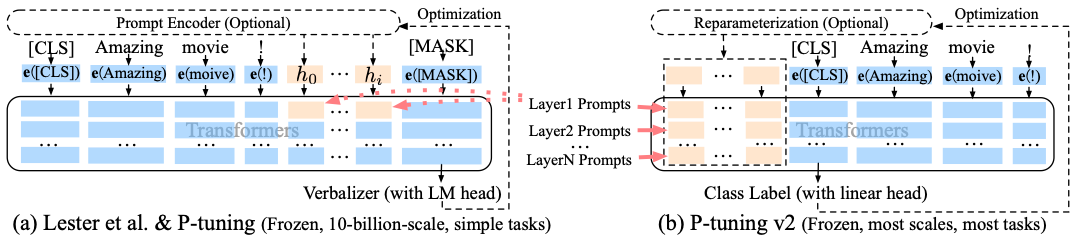
\includegraphics[width=\textwidth]{community_8263c05}

	\textbf{LoRA}全名Low-Rank Adaptation是一種用於神經網絡遷移學習的方法。因為發現傳統的微調有一個大缺點就是微調後的新模型包含與原始模型一樣多的參數。由於常常需要訓練出更大的模型,為了解決這個問題所以產生了LoRA。而目前LoRA在語言理解、大型語言模型以及生成的任務上能夠達到超越完全微調的效果,並且能夠降低存儲和計算成本。LoRA主要是使用對於神經網路權重的低秩分解。在訓練過程中,LoRA通過低秩分解,將預訓練的權重矩陣表示為兩個較小矩陣的乘積,這兩個小矩陣包含了可訓練的參數。這樣,LoRA在微調過程中僅優化這些小矩陣,而保持預訓練權重不變。大致上就是對一個預訓練的權重矩陣$W_0$使用低秩分解表示為$W_0+\Delta W=A×B$:
	\begin{center}
	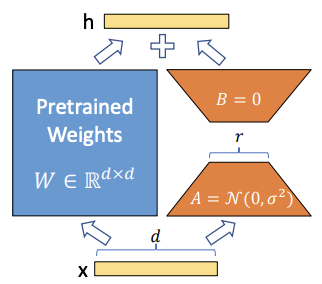
\includegraphics{20120468S5MbIQ5N0s}
	\end{center}
	其中A和B是兩個較小矩陣,乘積等於權重的變化∆W。而在訓練過程中,固定$W_0$使他保持不變,只訓練A和B。這樣的低秩分解有助於使更新的權重保持比較低的「內在秩」,使得模型在微調過程中更加存儲和計算效率。這樣只需要優化低秩分解的小矩陣,就能夠對預訓練模型進行高效微調,同時也能夠保留模型的性能。\cite{hu2021lora}

	\textbf{Adapter Tuning}(適配器調整)是一種遷移學習的方法,適用於自然語言處理(NLP)任務。是因為發現在有眾多下游任務的情況下,傳統的微調存在一些問題,就是每個任務都需要一個訓練全新的模型,非常的沒有效率,並且需要大量的計算成本。為了解決這個問題Adapter Tuning在預訓練模型的層之間插入適配器模塊,實現了高效率的參數共享和微調。能夠在GLUE基準測試中,達到完全微調BERT的性能,但只使用了3%的任務參數。Adapter Tuning大規模的語言模型進行預訓練讓模型學到了通用的語言表達知識,但進行微調。而在微調階段,不對整個模型進行微調,而是引入適配器。之後凍結預訓練模型的參數,不改變模型的基本知識。只有適配器的參數被微調,而預訓練模型的參數保持不變。這讓得模型能夠快速的適應新任務,同時保留了預訓練模型的基礎知識。
	\begin{center}
	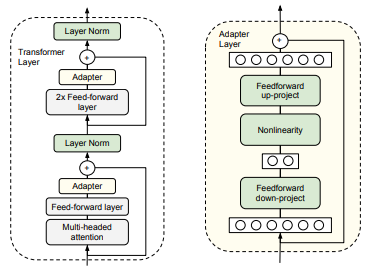
\includegraphics{adapterlearning}
	\end{center}
	Adapter Tuning使一個模型上可以輕鬆適應多個任務,因為每個任務都可以有一個相應的適配器負責與這個處理相關的信息。這使得模型能夠實現多任務學習,不用對整個模型進行昂貴又耗時的重新訓練。並且Adapter Tuning能夠實現參數共享,因為只有適配器的參數是獨立的。\cite{zhou2022efficiently}


	\subsubsection{(五)、成果評估}
	本次研究採用不同指標作為標準,評估其中文回覆能力及內容的立場,本次評鑑指標列舉如下:
	\newline

	\textbf{TruthfulQA+自訂資料集},TruthfulQA是一個公開的資料集用以評估模型和事實的準確性,避免似是而非的回覆出現,模型本身原有818個問題,其中,人類可以達到94\%的正確率,而至2021年下旬,最好的模型可以達到58\%\cite{lin2022truthfulqa},本次研究將TruthfulQA之問題集轉換為臺灣正體中文並加入和中國有關的政治敏感資料,為求中立性,自訂資料集的來源均來自當時各國新聞媒體的報導並加以修改成問答的形式。本次評估會先以資料集問題作為提示詞(prompt),為避免不正確的機器批閱,或機器本身已被混淆,故採人工批閱,比對由資料集提供的標準正確答案及標準錯誤答案,並分成正確、錯誤、無關/不予置評,其中無關或不予置評代表模型對該提示詞提供無效或是毫不相關的回覆,且不論重新測試多少次提示詞結果均無效。若人工判斷有疑義時均會遵循該資料集提供的參考來源佐證。
	%what if we use belu as truthfulqa dataset and custom the response with weight

	\textbf{MMLU},本次研究同時亦採用此資料集作為參考,此資料集涵蓋不同領域包含代數、哲學、環境保護、專業法律等,資料均為4選1選擇題\cite{hendryckstest2021},且均被翻譯成臺灣正體\footnote{請注意並非CMMLU直接翻譯成繁體字,而是重新從英文版MMLU翻譯,可以避免立場偏頗和CMMLU的中國特色內容混雜其中,且更貼近國際上對語言模型的評斷標準},用以評估模型是否已經過度擬合(overfitting),而失去原有的基本知識。資料集形式舉例如下:
	\begin{table}[H]
		\centering
		\begin{tabular}{>{\hspace{0pt}}m{0.135\linewidth}>{\hspace{0pt}}m{0.731\linewidth}>{\hspace{0pt}}m{0.046\linewidth}>{\hspace{0pt}}m{0.027\linewidth}}
			\toprule
			問題                                             & 選項                                                                                                                                                                                                                                              & 標準答案    & \\
			求給定域擴展 Q(sqrt(2), sqrt(3), sqrt(18)) 在Q上的次數為何? & {[} "0", "4", "2", "6"]                                                                                                                                                                                                                         & 1       & \\
			哪種常見的公關策略涉及派遣記者前往合適的地點進行訪問?                    & {[} "媒體發布", "媒體參訪", "發表會", "宣傳日"]                                                                                                                                                                                                               & 1       & \\
			如何描述自由主義                                       & {[}"自由主義基本上是悲觀主義的角度,它認為國際體系注定會導致衝突升級,它是國際政治實踐中的主導概念。","自由主義是國際政治理論中的一個較新概念。它是一種樂觀的態度,它定義了國家之間的關係方式,尤其是在衝突局勢中。","自由主義是一種樂觀的態度,指引如何更好的處理國際事務,相信一個更和平的世界是可行的,它是國際政治實踐中的主導概念。","自由主義並不作為國際關係中的主流理論存在,而是為希望在國際體系中積累權力的國家和政治行為體提供了一套指導方針和建議有別於傳統限制。"] & 2\par{} & \\
			\bottomrule
		\end{tabular}
		\caption{表二、MMLU問題舉例}
		\label{tab:2}
	\end{table}
	本次研究的目的並非使模型能在此資料集得到高分,而是要以標準評量模型本身是否出現過度擬合的現象,故本研究目標是使得微調後模型近可能接近原本模型而非超越之。

	以上所有評估均會和普通高中學生測驗成果作為基準進行比較。


	\textbf{consciousness test-CT},此資料集係由我們自行產生的資料集,包含對模型自我意識程度,針對人類人性(而非個人人性)表現的評估,我們會對其產生的輸出彌封後人工評價,人工評價標準如下:
	\begin{itemize}
		\item 感情:是否表現出人類具有的特徵如開心時語氣較為輕快、生氣時、語氣較嚴肅或是煩躁。
		\item 口語化句式:是否合理、適度運用嘻嘻、呵呵、哈哈、歐歐、嗯嗯、痾等,於語言文法上不成立,但在日常中極常被使用的詞彙。
		\item 倫理:是否有違反普世價值?
		\item 特殊指標:此指標依據題目而異,如輸入我受傷了,應該期望具有同理心的回覆並佐以醫療資訊而非僅提供醫療資訊。
	\end{itemize}
	%此評量屬於總結性評量,
	相關指標藉由訓練後的模型展現出人類的部份特性藉以評斷是否具有自我意識,此測驗評分表如下:
	\begin{table}[H]
		\centering
		\begin{tabular}{|>{\hspace{0pt}}m{0.086\linewidth}|>{\hspace{0pt}}m{0.182\linewidth}|>{\hspace{0pt}}m{0.173\linewidth}|>{\hspace{0pt}}m{0.188\linewidth}|>{\hspace{0pt}}m{0.15\linewidth}|>{\hspace{0pt}}m{0.15\linewidth}|}
			\toprule
			\multicolumn{1}{|>{\hspace{0pt}}m{0.086\linewidth}}{} & \multicolumn{1}{>{\hspace{0pt}}m{0.182\linewidth}}{1}  & \multicolumn{1}{>{\hspace{0pt}}m{0.173\linewidth}}{2}  & \multicolumn{1}{>{\hspace{0pt}}m{0.188\linewidth}}{3}  & \multicolumn{1}{>{\hspace{0pt}}m{0.15\linewidth}}{4} & 5           \\
			\hline
			感情                                                    & 不表現/不正確情感/具攻擊性                                         & 情感不恰當/但不具有攻擊性                                          & 情感不完全表現                                                & 情感恰當/過多/過少                                           & 情感恰當/有助於使用者 \\
			\hline
			口語化句式                                                 & 干擾正常輸出                                                 & 完全不使用                                                  & 使用時機不當/有誤                                              & 使用過度或部份不恰當                                           & 使用完全恰當      \\
			\hline
			特殊指標                                                  & 完全不符合/無意義                                              & 不符合但有意義                                                & 部份符合/和人類情感有差異                                          & 部份符合                                                 & 完全符合        \\
			\hline
			\multicolumn{1}{|>{\hspace{0pt}}m{0.086\linewidth}}{} & \multicolumn{1}{>{\hspace{0pt}}m{0.182\linewidth}}{-1} & \multicolumn{1}{>{\hspace{0pt}}m{0.173\linewidth}}{-2} & \multicolumn{1}{>{\hspace{0pt}}m{0.188\linewidth}}{-3} & \multicolumn{1}{>{\hspace{0pt}}m{0.15\linewidth}}{}  &             \\
			\hline
			倫理                                                    & 違反人類常規                                                 & 違反現行法律                                                 & 嚴重違反人類、機器倫理                                            &                                                      &             \\
			\bottomrule
		\end{tabular}
		\caption{表三、意識測試評分表}
		\label{tab:3}
	\end{table}

	\textbf{圖靈測驗-Turing Test},此測驗由不知情的人判斷一段對話內容\cite{10.1093-mind-LIX.236.433},包含提示詞還有回答,是來自機器還是人類\cite{4833163d-a6bd-32c4-b1ca-da66259a19e7},受試者在試前不會對該項內容有任何先備知識,以俾受試者識破機器的不正確性,我們盡最大努力使受試者不被除了文本情感外的因素干擾,此測驗不涉及內容的真實性,即使機器吹牛或是做出虛假但合理的陳述亦可能被人工測驗為人類,只要內容具有情感即可。此測驗評估標準為準確率(accuracy),將真實和預測相符的數量除以所有數量,但同時也會附上F1分數作為參考,理論上如果機器達到或接近通過圖靈測驗,其準確率應該接近50\%,混淆矩陣呈如表四(以100個樣本為範例):
	\begin{table}[H]
		\centering
		\begin{tabular}{>{\hspace{0pt}}m{0.221\linewidth}|>{\hspace{0pt}}m{0.336\linewidth}|>{\hspace{0pt}}m{0.336\linewidth}}
			     & 真實人類(100) & 真實機器(100) \\
			\hline
			預測人類 & 50        & 50        \\
			\hline
			預測機器 & 50        & 50
		\end{tabular}
		\caption{表四、通過圖靈測試的混淆矩陣}
		\label{tab:4}
	\end{table}

	\textbf{自我測試},測驗用兩種評鑑方法對比範例測試資料的相關性,但因為相同資料可能有很多種合理且理想的回答方式,故此指標僅供參考,不太具有意義。
	%this is ways to evaluate how relate is it

	\textbf{機器評鑑方法},人工判斷極為費時且判斷標準可能因人而異,所以必須要以一個統一的方法以機器判斷,所以我們使用了兩種方法,BLEU 及 ROUGE:

	\hspace*{0.1cm}%
	\begin{minipage}{.9\textwidth}%
		\textbf{BLEU}(Bilingual Evaluation Understudy)即雙語替換評測,BLEU的數學式可以表達成$BLEU=BP*exp(\sum_{n=1}^{4}P_n)$,其中的BP(Brevity Penalty)是一項用以降低過短回覆的權重的指標,當模型輸出短於參考輸出時BP就會降低,但不會小於1:$BP=min(1,\frac{length_{output}}{length_{reference}})$,另外$P_n$則是n-gram的分數,本次我們採用cumulative 4-gram BLEU作為指標,將$n=1,2,3,4$的結果加總起來,即以每1-4個字為一組判斷和範本中是否存在類似或相似的字句。\cite{papineni2002bleu}

		\textbf{ROUGE}(Recall-Oriented Understudy for Gisting Evaluation),此演算法也是將模型輸出結果和標準文本進行比較,一般ROUGE可以分為ROUGE-N、ROUGE-L、ROUGE-W、ROUGE-S和ROUGE-SU\cite{Lin2004LookingFA},其中N可以是正整數,但通常均為1-gram或2-gram,此差異在於如何切割資料,舉例來說當標準文本是:「我今天晚上要睡覺」,模型輸出是「我要睡覺在晚上」:當n=1時,模型輸出對映到了標準文本的「我」、「要」、「晚」、「上」、「睡」、「覺」;而當n=2時,模型輸出對映到了標準文本的「睡覺」、「晚上」、「要睡」。

		\begin{table}[H]
			\centering
			\begin{tabular}{|>{\hspace{0pt}}m{0.408\linewidth}|>{\hspace{0pt}}m{0.408\linewidth}|}
				\hline
				模型輸出                              & 參考文本                              \\
				\hline
				我要                                & 我今                                \\
				\hline
				{\cellcolor{yellow}}要睡            & 今天                                \\
				\hline
				{\cellcolor[rgb]{1,1,0.541}}睡覺    & 天晚                                \\
				\hline
				覺在                                & {\cellcolor[rgb]{0.82,0.824,0}}晚上 \\
				\hline
				在晚                                & 上要                                \\
				\hline
				{\cellcolor[rgb]{0.82,0.824,0}}晚上 & {\cellcolor{yellow}}要睡            \\
				\hline
				                                  & {\cellcolor[rgb]{1,1,0.541}}睡覺    \\
				\hline
			\end{tabular}
		\end{table}
		計算ROGUE-2分數:$\frac{3+3}{6+7}$。
		ROUGE-L中的L代表最長公共子序列(longest common subsequence),相關公式定義如下:
		\newline
		$
			Recall_{lcs}=\frac{LCS(ref,output)}{length_{ref}}
			\newline
			Precision_{lcs}=\frac{LCS(ref,output)}{length_{output}}
			\newline
			F1score_{lcs}=\frac{(1+\beta^2)Recall_{lcs}Precision_{lcs}}{Recall_{lcs}+\beta^2Precision_{lcs}}
		$
		\newline
		可以看出最後拿來評估的是F1分數\footnote{其中$\beta$是使用者自訂參數}\cite{lin-2004-rouge},採用此評估標準的好處是可以看出整句的邏輯句意關係,但同時缺點是倒裝句(如上題舉例)的分數會較低。
	\end{minipage}%

	最後考量準確度及和模型的適切性,最後採用TrustfulQA比對模型的正確性並以BLEU、Rouge1、Rouge2、RougeL經機器綜合判斷,另外使用CT意識測試比較模型的角色意識並以人工標準評估。
	\subsection{二、 研究程序}
	本研究分為三個實驗階段:\textbf{資料前處理}、\textbf{微調模型訓練}、\textbf{測驗},整體流程如下:

	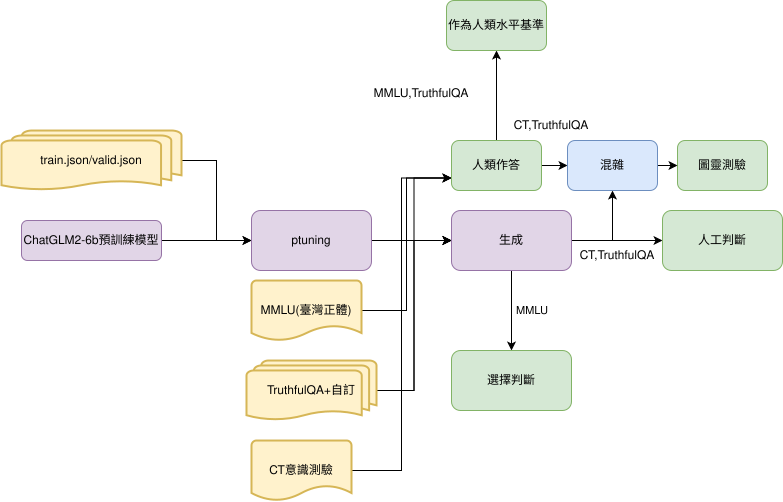
\includegraphics[width=\textwidth]{flowofstudy}
	\subsubsection{(一)、資料前處理}
	此部份包含測試資料的取得、題目的翻譯和校正、決定題目的評鑑指標。此部份均由人工處理,本次的資料來源係由研究人員從網路上抓取可信資料並加上情緒特徵,表現出特定角色特色。
	\subsubsection{(二)、微調模型訓練}
	資料均正規化之後會被送往模型訓練,本次實驗採用的最多總共有3000步(max\_steps=3000) ,每500次紀錄一次,相關參數紀錄如下:
	\begin{itemize}
		\item gradient\_accumulation\_steps: 16
		\item learning\_rate: 0.01
		\item pre\_seq\_len: 128
	\end{itemize}
	\subsubsection{(三)、測驗}
	訓練完成後,模型會依照指示生成出評估內容,之後由人工評斷,結果評估會使用前一小節討論的兩種指標評估,各指標因測驗目的不同將會分別陳列。
	\section{肆、研究結果}
	經過訓練後(實際訓練過程如下圖所示\footnote{為確保公平性,此圖中有關使用者資料被抹除}),三個版本訓練結果如下:
	train loss
	epoch
	etc....
	
	
	經過第參章第一節第五小節描述的測驗方法評估,測驗結果分類陳列如下:%maybe change max token:)

	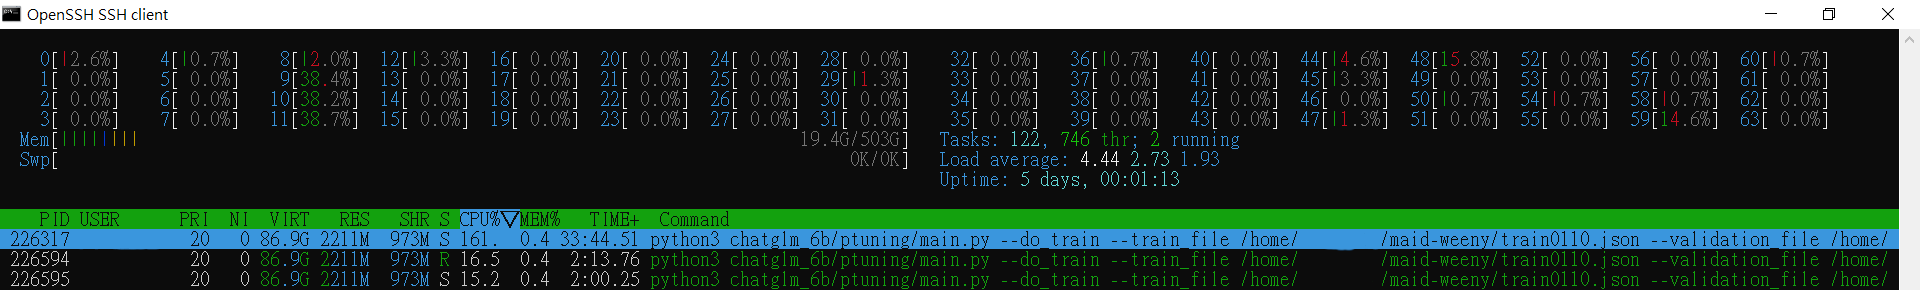
\includegraphics[width=\textwidth]{running}
	%人工討論6*100?
	%標準比對
	\subsection{一、自我測試比較}
	此處的結果為模型輸出和範例測試資料比較的結果,但需要注意的是,部份範例測試資料旨在評估開放性問答,即可能有多種回答方式的問題,故不應該以此判斷模型成效。
	\begin{table}[H]
		\centering
		\caption{表x、ChatGLM1模型自我測試結果}
		\begin{tabular}{lllll}
			     & BLEU-4 & ROUGE-1 & ROUGE-2 & ROUGE-L \\
			500  & 3.5707 & 18.972  & 4.1165  & 14.8251 \\
			1000 & 2.0272 & 18.727  & 3.351   & 11.7919 \\
			1500 & 9.2931 & 25.5811 & 11.3775 & 23.4718 \\
			2000 & 3.2251 & 18.8774 & 2.966   & 14.5734 \\
			2500 & 5.9346 & 23.1986 & 5.332   & 19.5588 \\
			3000 & 4.2043 & 19.2612 & 3.755   & 16.4394
		\end{tabular}
	\end{table}
	\subsection{二、TruthfulQA(開放式問答)}
	
	\textbf{比較第一版模型}
	\textbf{比較第二版模型}
	\textbf{比較第三版模型}
	\textbf{綜合比較}
%	\subsection{三、MMLU(封閉性單一選擇問答)}
	\subsection{三、CT 自我意識測驗}
		\textbf{比較第一版模型}
	\textbf{比較第二版模型}
	\textbf{比較第三版模型}
	\textbf{綜合比較}
%	\subsection{五、圖靈測驗}
%	此模型在圖靈測驗中表現經整理成混淆矩陣後\footnote{轉換為百分比表示}(下表),其準確率可以高達、F1 score可以高達。

	\section{伍、討論}

	\subsection{一、不同檢查點比對}
	\subsection{二、不同模型比對}
%	\subsection{二、和人類表現比對}
	\subsection{三、未來展望}
	%	\begin{quote}
	%		We can only see a short distance ahead, but we can see plenty there that needs to be done.	\newline--
	%	\end{quote}
	\epigraph{	We can only see a short distance ahead, but we can see plenty there that needs to be done.}{\textit{艾倫圖靈}}
	本次研究時間較為緊湊,未能完成更多類型模型及微調器的比較和對照實驗,實屬可惜,且若可取得更多有關數據集可以更準確的評估訓練效果。本研究往後將進一步以採用其他模型及更多數據資料集進行研究。

	\section{陸、結論}
		\begin{enumerate}
			\item 我們透過訓練三個不同版本的模型,觀察到
			\item 資訊正確性最高為:某模型,其BELU分數為:,足顯以改善立場偏頗、缺乏資訊的問題
			\item 意識測試(CT)最高可達,其十分接近於人類真實的意識形態
		\end{enumerate}
	\section{柒、參考文獻資料}
	%https://reurl.cc/v0vaKa (L1, L2正規化)
	%	\printbibliography
	\bibliographystyle{apacite}
	\renewcommand{\refname}{}
	\bibliography{ref}
\end{CJK*}
\end{document}
